%%%%%%%%%%%%%%%%%%%%%%%%%%%%%%%%%%%%%%%%%%%%%%%%%%%%%%%%%%%%%%%%%%%%%%%%
%% -----------------  Drawings portion of the patent  --------------- %%
%%                                                                    %% 
%% NOTES:                                                             %%
%% do drawings with any drawing software, i.e. xfig, photoshop        %%
%% save drawing in eps format with tight bounding box option enabled  %%

\begin{figure}[h]
\centering
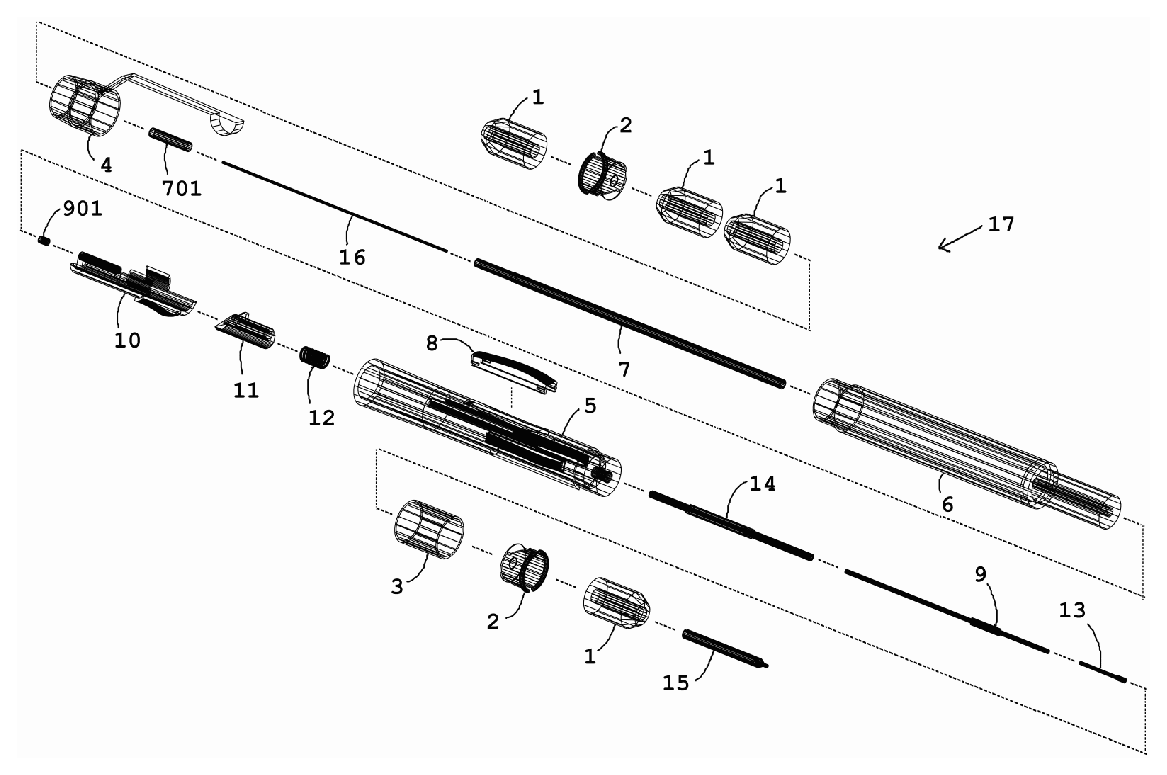
\includegraphics[width=\textwidth]{drawings/assembly3-labeled.ps}
\caption{\prior\label{fig:assembly}}
\end{figure}

\begin{figure}[h]
\centering
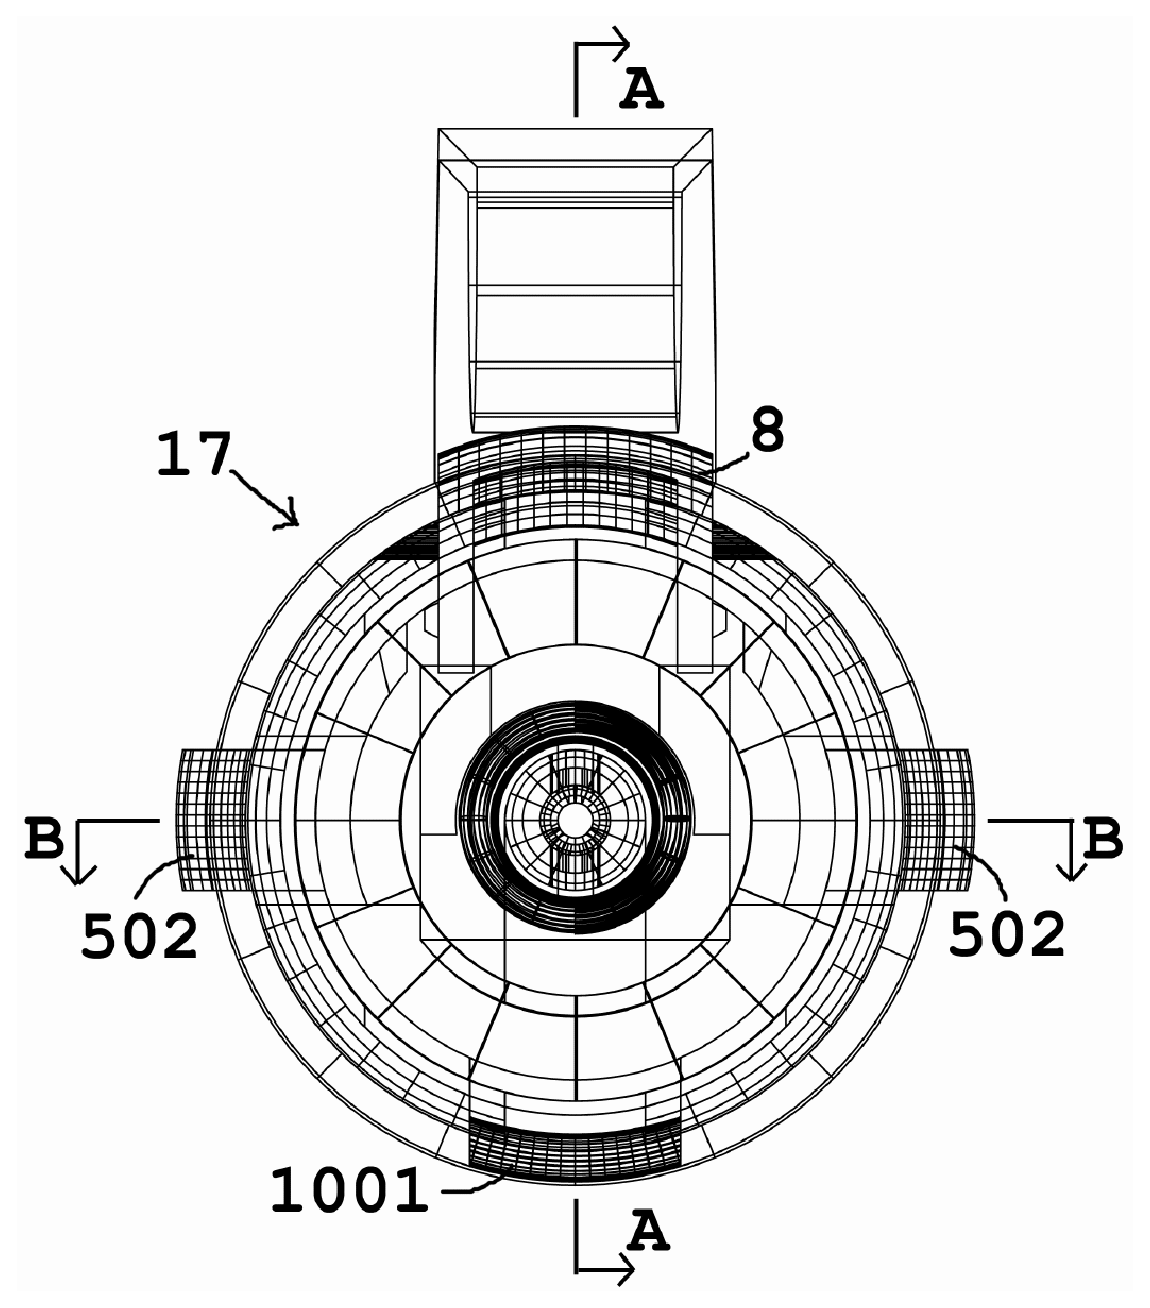
\includegraphics[width=2.4in]{drawings/front-labeled.ps}
\caption{\label{fig:front}}
\end{figure}

\begin{sidewaysfigure}[h]
\centering{%
  \hspace{-.3in}
  \subfloat[\label{fig:cross-side-normal}]{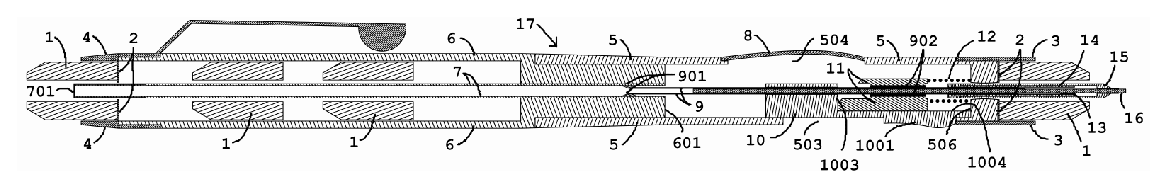
\includegraphics{drawings/cross-side-normal-labeled.ps}}
  \\
  \vspace{.5in}
  \hspace{-.3in}
  \subfloat[\label{fig:cross-side-advance}]{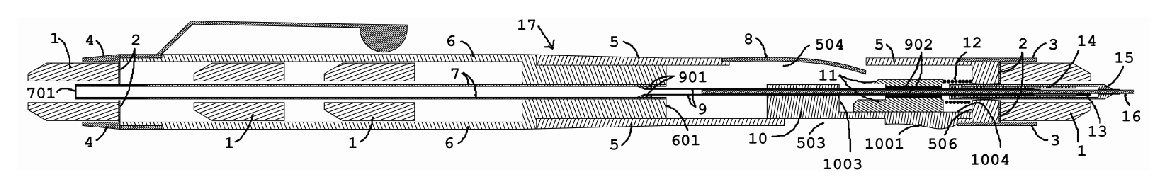
\includegraphics{drawings/cross-side-advance-labeled.ps}}
  \\
  \vspace{.5in}
  \hspace{-.3in}
  \subfloat[\label{fig:cross-side-retract}]{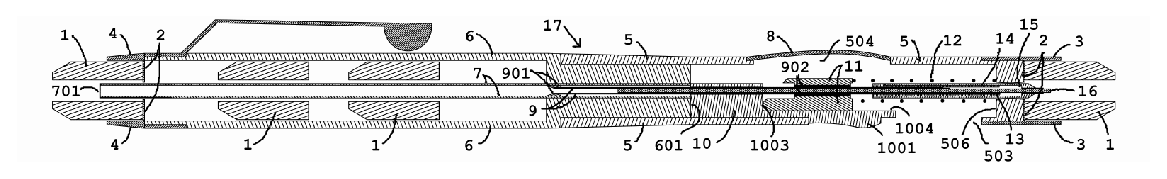
\includegraphics{drawings/cross-side-retract-labeled.ps}}
  \\
}
\addtocounter{figure}{1} %% Required for subfloats 
\setcounter{subfigure}{0} %% Required for subfloats
\end{sidewaysfigure}

